\section{Auswertung}
\label{sec:Auswertung}

\subsection{Statische Methode}
Zunächst wird in diesem Abschnitt die statische Methode behandelt.

\begin{figure}
    \centering
    \caption{Vier Temperaturverläufe von unterschiedlichen Materialien.}
    \begin{subfigure}{\textwidth/2}
        \centering
        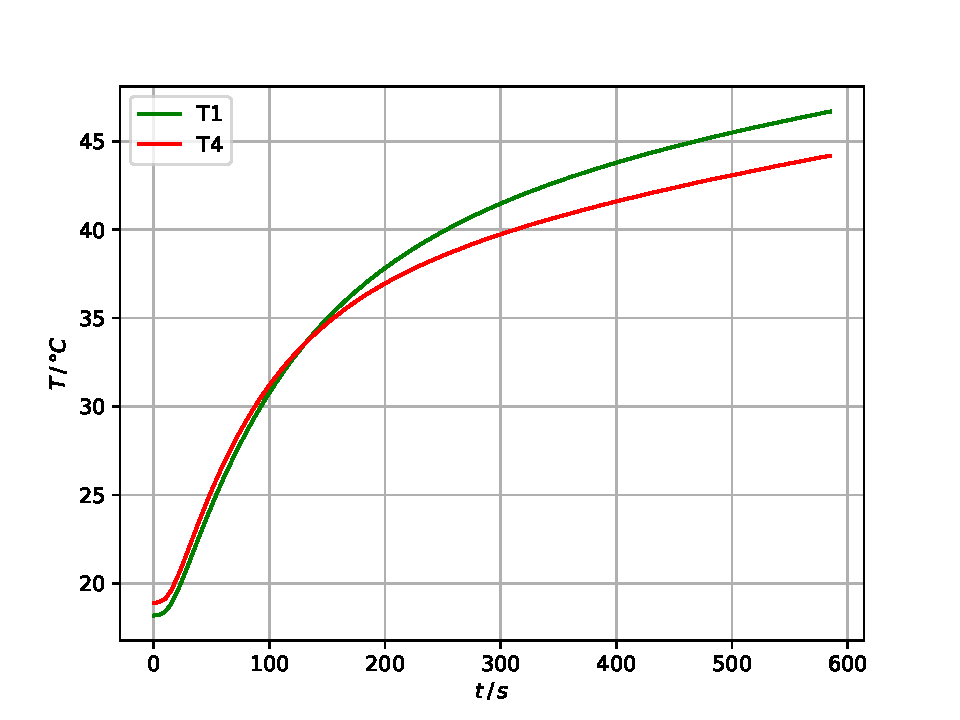
\includegraphics[width=\textwidth]{content/data/statsisch_T1_T4.pdf}
        \caption{Der Temperaturverlauf an Thermoelemt 1 und 4.}
        \label{fig:stat_1_4}
    \end{subfigure}
    \begin{subfigure}{\textwidth/2}
        \centering
        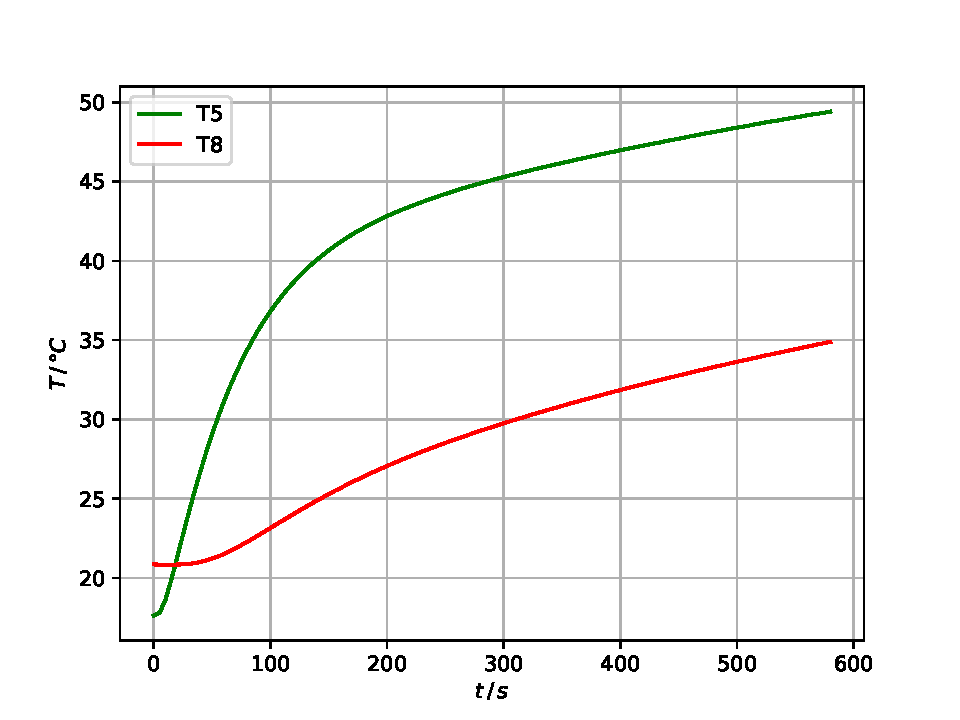
\includegraphics[width=\textwidth]{content/data/statsisch_T5_T8.pdf}
        \caption{Der Temperaturverlauf an Thermoelement 5 und 8.}
        \label{fig:stat_5_8}
    \end{subfigure}
    \label{fig:stat}
\end{figure}

Die aufgenommenen Temperaturverläufe sind in Abbildung \ref{fig:stat} zu finden.
Es fällt auf, dass alle Temperaturen einem exponentiellem Wachstum folgen.
Nach einer Zeit von $\SI{150}{\second}$ nimmt dieses aber stark ab und die Temperaturen streben gegen einen Sättigungswert.
Dieser Wert ist bei jedem Material anders, die hier aufgenommenen Temperaturen nach $\SI{590}{\second}$ sind: 
\begin{align*}
    T_1 = \SI{46.59}{\celsius} \\
    T_4 = \SI{44.04}{\celsius} \\
    T_5 = \SI{48.82}{\celsius} \\
    T_8 = \SI{34.98}{\celsius} \\
\end{align*}

Die höchste Temperatur erreicht hier das Thermoelement 5.
Der dazu gehörige Stab besteht aus Aluminium.
\FloatBarrier
Nun soll die Wärme berechnet werden die in der Zeit $t$ durch zwei der Stäbe geflossen ist.
Dazu wird \eqref{eqn:leit} genutzt.
Die nötigen Wärmeleitfähigkeiten der beiden Metalle werden dabei aus der Quelle \cite{leitfaehigkeit} entnommen.
Die Abmessung der Stäbe sind in \cite{anleitung} zu finden.
Der Abstand zwischen den Thermoelementen ist jeweils $\SI{3}{\centi\meter}$.
In der Tabelle \ref{tab:waerme_diff} sind die berechneten Ergebnisse zu finden.
\begin{table}
\centering
\caption{Die Wärmedifferenz der verschiedenen Thermoelemente des Stabes.}
    \begin{tabular}{S S S}
    \toprule
    $t \, / \, \si{\second}$ & $\frac{\delta Q_{21} }{\delta t} \, / \, \si{\watt}$ & $\frac{\delta Q_{87} }{\delta t} \, / \, \si{\watt}$ \\
    \midrule
    50 & -1.235 & -0.279 \\
    150 & -0.768 &  -0.405\\
    250 & -0.531 & -0.374 \\
    350 & -0.433 & -0.351 \\
    450 & -0.395 & -0.337 \\
    \bottomrule 
    \end{tabular}
\label{tab:waerme_diff}
\end{table}

Aus der Temperaturdifferenz von $T_1$ und $T_2$ sowie $T_7$ und $T_8$ ergeben sich außerdem zwei Graphen.
Diese sind in Abbildung \ref{fig:stat_vergleich} zu sehen.

\begin{figure}
\centering
\caption{Die Temperaturdifferenzen der vier gemessenen Temperaturen.}
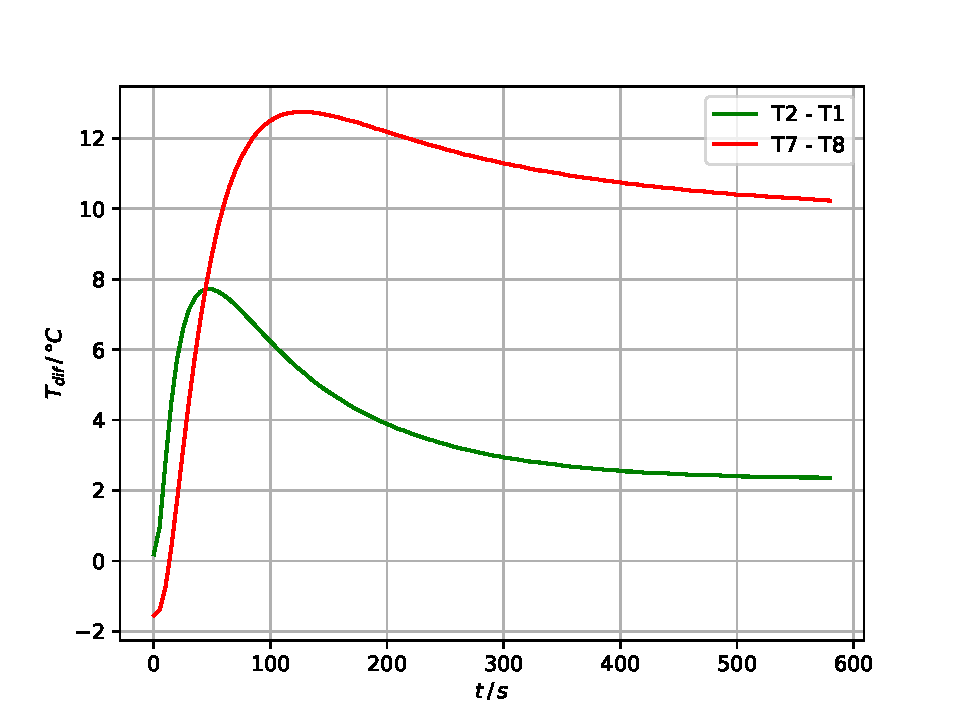
\includegraphics[width = 0.8\textwidth]{content/data/statsisch_vergleich.pdf}
\label{fig:stat_vergleich}
\end{figure}
\FloatBarrier

\subsection{Dynamische Methode}

Nun soll mit den, durch die dynamische Methode ermittelten Werten, die Wärmeleitfähigkeit $\kappa$ von Edelstahl und Messing ermittelt werden.
Die Temperaturverläufe an den Thermoelementen dieser beiden Stäbe sind in Abbildung \ref{fig:dyn} zu finden
\begin{figure}
    \centering
    \caption{Zwei Temperaturverläufe von zwei Metallen.}
    \begin{subfigure}{\textwidth/2}
        \centering
        \caption{Der Temperaturverlauf der beiden Thermoelemente des Messingstabes.}
        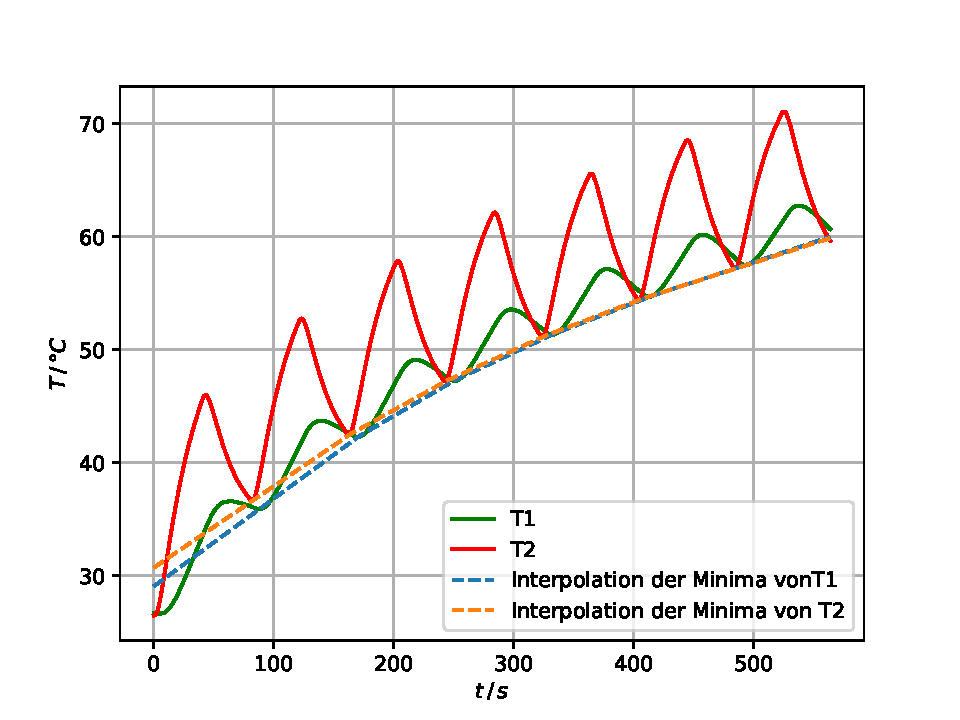
\includegraphics[width = \textwidth]{content/data/dynamisch_T1_T2.pdf}
        \label{fig:dyn_T1_T2}
    \end{subfigure}
    \begin{subfigure}{\textwidth/2}
        \centering
        \caption{Der Temperaturverlauf an den beiden Thermoelementen des Edelstahlstabes.}
        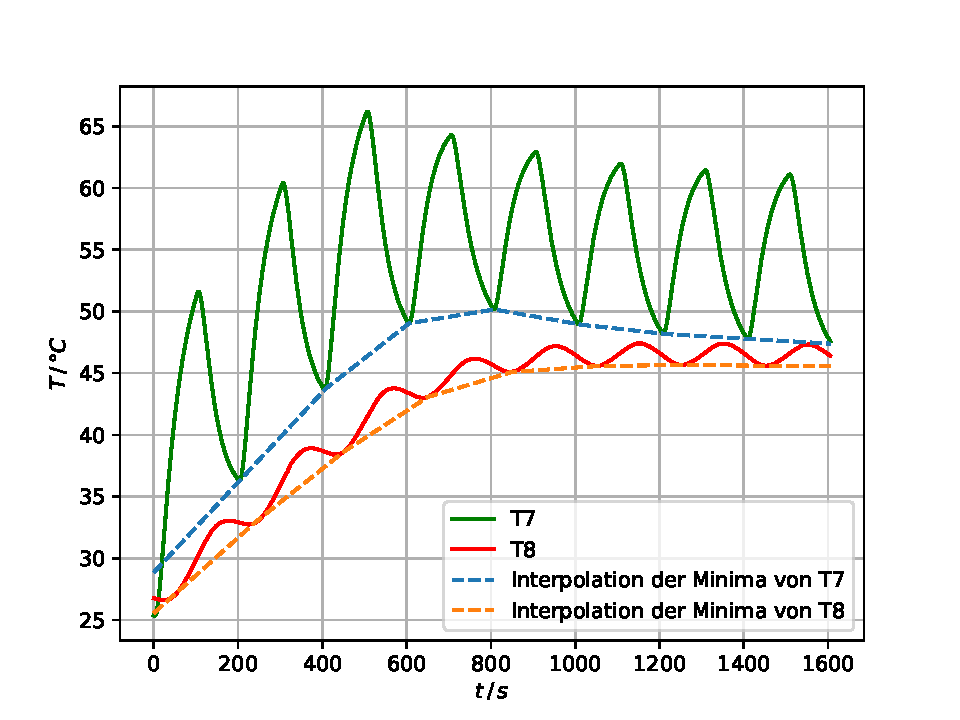
\includegraphics[width=\textwidth]{content/data/dynamisch_T7_T8.pdf}
        \label{fig:dyn_T7_T8}
    \end{subfigure}
\label{fig:dyn}
\end{figure}

%In die Disskusion schreiben, dass die vierte amplitude wesentlich kleiner ist als die dritte, da wir spannung runter regeln mussten

Zu erwähnen ist, dass die Periodendauer, welche zum Aufnehmen der Werte für Abbildung \ref{fig:dyn_T1_T2}, $\SI{80}{\second}$ beträgt wohingegen die Periodendauer der anderen Abbildung $\SI{200}{\second}$ beträgt.
Die Interpolationen, der Minima aller Graphen wurden mit der Python Bibliothek scipy \cite{scipy} durchgeführt.
Durch diese wurde eine Funktion erstellt, welche die Minima interpoliert.
Mit dieser Funktion kann wiederrum die absolute Amplitude der Temperaturen berechnet werden.
Mit \eqref{eqn:kappa} wird nun die Wärmeleitfähigkeit der beiden Metalle bestimmt.
Dabei wurden die Dichte der beiden Metalle, sowie die spezifische Wärmekapazität aus \cite{anleitung} entnommen.
Der Abstand $\Delta x$ zwischen den Thermoelementen beträgt $\SI{3}{\centi\meter}$.
Die Tabelle \ref{tab:erg_mess} zeigt die Amplituden und die Phasenverschiebung der Wärmekurve des Messings, sowie die damit berechnete Wärmeleitfähigkeit.
\begin{table}
\centering
\caption{Die berechneten absoluten Amplituden und der Phasenunterschied der Temperaturwelle von Messing, sowie dessen Wärmeleitfähigkeit.}
\begin{tabular}{cccc}    
    \toprule
    $A_\text{nah} \,/\, \si{\celsius}$ & $A_\text{fern} \,/\, \si{\celsius}$ & $\Delta t \,/\, \si{\second}$ & $\kappa \, / \, \si{\frac{\watt}{\meter\kelvin}}$ \\
    \midrule
    12.186 & 2.632 & 20 & 47.156 \\
    13.178 & 3.858 & 16 & 73.540 \\
    13.010 & 3.852 & 15 & 79.171 \\
    12.970 & 3.925 & 14 & 86.388 \\
    12.784 & 3.923 & 13 & 94.122 \\
    12.752 & 3.923 & 13 & 94.328 \\
    12.527 & 3.673 & 13 & 90.639 \\
    \bottomrule
\end{tabular}
\label{tab:erg_mess}
\end{table}
\FloatBarrier
Im Mittel ergibt sich für Messing eine Wärmeleitfähigkeit von 
\begin{equation*}
    \kappa = \SI{80.763(6316)}{\frac{\watt}{\meter\kelvin}} .
\end{equation*}
Zur Mittelung der Werte aus Tabelle \ref{tab:erg_mess} wird die Numpy Funktion 'mean' genutzt \cite{numpy}.
Zur Berechung des Fehlers des Mittelwertes wird die scipy Funktion 'sem' genutzt \cite{scipy}.
Zusätzlich wird die Wärmeleitfähigkeit von Aluminium bestimmt. Die dazu gemessenen Werte sind in Tabelle \ref{tab:erg_alu} zu finden.
Die benötigten Literaturwerte wurden aus \cite{anleitung} entnommen. Auch hier ist der Abstand zwischen den Thermoelementen $\SI{3}{\centi\meter}$.

\begin{table}
\centering
\caption{Die berechneten absoluten Amplituden, sowie die jeweiligen Phasenverschiebungen und die Wärmeleitfähigkeit von Aluminium.}
    \begin{tabular}{cccc}
    \toprule
    $A_\text{nah} \,/\, \si{\celsius}$ & $A_\text{fern} \,/\, \si{\celsius}$ & $\Delta t \,/\, \si{\second}$ & $\kappa \, / \, \si{\frac{\watt}{\meter\kelvin}}$ \\
    \midrule
    14.588 & 3.183 & 10 & 68.769 \\
    16.366 & 7.122 & 8  & 157.121 \\
    16.025 & 7.692 & 8  & 178.114 \\
    15.946 & 7.689 & 7  & 205.134 \\
    15.608 & 7.577 & 6  & 239.665 \\
    15.668 & 7.548 & 7  & 204.577 \\
    15.421 & 7.308 & 7  & 200.087 \\
    \bottomrule
    \end{tabular}
\label{tab:erg_alu}
\end{table}
Durch die Werte aus der Tabelle \ref{tab:erg_alu} ergibt sich für die Wärmeleitfähigkeit des Aluminiums ein Wert von 
\begin{equation*}
    \kappa = \SI{179.071(20751)}{\frac{\watt}{\meter\kelvin}} .
\end{equation*}
\FloatBarrier
Die letzte Messreihe die ausgewertet wird ist die des Edelstahls.
Die Werte dazu sind in Tabelle \ref{tab:erg_edel} zu finden. Sie zeigt die Amplituden und den Phasenunterschied der Wärmekurve des Edelstahls.
\begin{table}
\centering
\caption{Die berechnteten absoluten Amplituden, der Phasenunterschied und die jeweilige Wärmeleitfähigkeit von Edelstahl.}
\begin{tabular}{cccc}
    \toprule
    $A_\text{nah} \,/\, \si{\celsius}$ & $A_\text{fern} \,/\, \si{\celsius}$ & $\Delta t \,/\, \si{\second}$ & $\kappa \, / \, \si{\frac{\watt}{\meter\kelvin}}$ \\
    \midrule
    18.873 & 2.284 & 62 & 10.998 \\
    20.323 & 2.587 & 57 & 12.257 \\
    19.796 & 2.561 & 60 & 11.735 \\
    14.695 & 2.018 & 50 & 14.508 \\
    13.356 & 1.836 & 48 & 15.119 \\
    13.399 & 1.790 & 44 & 16.260 \\
    13.470 & 1.763 & 41 & 17.275 \\
    13.530 & 1.754 & 41 & 17.191 \\
    \bottomrule
\end{tabular}
\label{tab:erg_edel}
\end{table}

Im Mittel ergibt sich aus den Werten der Tabelle \ref{tab:erg_edel} eine Wärmeleitfähigkeit von
\begin{equation*}
    \SI{14.418(879)}{\frac{\watt}{\meter\kelvin}}
\end{equation*} 
für Edelstahl.

\FloatBarrier